% Options for packages loaded elsewhere
\PassOptionsToPackage{unicode}{hyperref}
\PassOptionsToPackage{hyphens}{url}
%
\documentclass[
]{article}
\usepackage{lmodern}
\usepackage{amsmath}
\usepackage{ifxetex,ifluatex}
\ifnum 0\ifxetex 1\fi\ifluatex 1\fi=0 % if pdftex
  \usepackage[T1]{fontenc}
  \usepackage[utf8]{inputenc}
  \usepackage{textcomp} % provide euro and other symbols
  \usepackage{amssymb}
\else % if luatex or xetex
  \usepackage{unicode-math}
  \defaultfontfeatures{Scale=MatchLowercase}
  \defaultfontfeatures[\rmfamily]{Ligatures=TeX,Scale=1}
\fi
% Use upquote if available, for straight quotes in verbatim environments
\IfFileExists{upquote.sty}{\usepackage{upquote}}{}
\IfFileExists{microtype.sty}{% use microtype if available
  \usepackage[]{microtype}
  \UseMicrotypeSet[protrusion]{basicmath} % disable protrusion for tt fonts
}{}
\makeatletter
\@ifundefined{KOMAClassName}{% if non-KOMA class
  \IfFileExists{parskip.sty}{%
    \usepackage{parskip}
  }{% else
    \setlength{\parindent}{0pt}
    \setlength{\parskip}{6pt plus 2pt minus 1pt}}
}{% if KOMA class
  \KOMAoptions{parskip=half}}
\makeatother
\usepackage{xcolor}
\IfFileExists{xurl.sty}{\usepackage{xurl}}{} % add URL line breaks if available
\IfFileExists{bookmark.sty}{\usepackage{bookmark}}{\usepackage{hyperref}}
\hypersetup{
  pdftitle={Neural\_Net\_Basics},
  hidelinks,
  pdfcreator={LaTeX via pandoc}}
\urlstyle{same} % disable monospaced font for URLs
\usepackage[margin=1in]{geometry}
\usepackage{graphicx}
\makeatletter
\def\maxwidth{\ifdim\Gin@nat@width>\linewidth\linewidth\else\Gin@nat@width\fi}
\def\maxheight{\ifdim\Gin@nat@height>\textheight\textheight\else\Gin@nat@height\fi}
\makeatother
% Scale images if necessary, so that they will not overflow the page
% margins by default, and it is still possible to overwrite the defaults
% using explicit options in \includegraphics[width, height, ...]{}
\setkeys{Gin}{width=\maxwidth,height=\maxheight,keepaspectratio}
% Set default figure placement to htbp
\makeatletter
\def\fps@figure{htbp}
\makeatother
\setlength{\emergencystretch}{3em} % prevent overfull lines
\providecommand{\tightlist}{%
  \setlength{\itemsep}{0pt}\setlength{\parskip}{0pt}}
\setcounter{secnumdepth}{-\maxdimen} % remove section numbering
\ifluatex
  \usepackage{selnolig}  % disable illegal ligatures
\fi

\title{Neural\_Net\_Basics}
\author{}
\date{\vspace{-2.5em}}

\begin{document}
\maketitle

\hypertarget{review-of-a-derivative}{%
\subsubsection{Review of a Derivative}\label{review-of-a-derivative}}

\textbf{Question !} What is the derivative of the function \(f(x) = 3x\)
with respect to (w.r.t.) \(x\)?

\textbf{Question !} What is the derivative of the function
\(f(x) = 3x^2\) w.r.t. \(x\)?

\textbf{Question !} What does the derivative signify?

\hypertarget{review-of-the-chain-rule-in-1-dimension}{%
\subsubsection{Review of the Chain Rule (in
1-Dimension)}\label{review-of-the-chain-rule-in-1-dimension}}

Again, let \(f(x) = 3x^2\). But now, let x itself be a function which
depends on another variable \(y\). Suppose this function is
\(x = \frac{1}{2}y\)

\textbf{Question !} First, verify that if you substitute in
\(\frac{1}{2}y\) for \(x\) into the initial equation \(f(x)\), then take
the derivative w.r.t. \(y\), you get \(\frac{df}{dy} = \frac{3}{2}y\)

The \textbf{Chain Rule} states the following: For some function \(f\)
depending on \(x\), which itself is a function which depends on \(y\),
then \ldots{} \[ 
\frac{df}{dy} = \frac{df}{dx} \frac{dx}{dy}
\]

\textbf{Question !} Use the Chain Rule to verify that
\(\frac{df}{dy} = \frac{3}{2}y\).

\hypertarget{review-of-the-chain-rule-in-multi-dim}{%
\subsubsection{Review of the Chain Rule (in
Multi-Dim)}\label{review-of-the-chain-rule-in-multi-dim}}

We will now verify the multi-variable/multi-dimension version of the
Chain Rule with an example. This is needed to solve problems related to
the Back-Propagation Algorithm later on.

Consider a function \(f\) that depends on \(x\) and \(y\) as follows.
\(f := f(x,y) = 3x^2 + y\)

Let \(x\), \(y\) both be functions of a variable \(t\), \(x(t) = 2t\)
and \(y(t) = t^2\).

Our goals is to solve for the derivative of \(f\) w.r.t. \(t\), aka
\(\frac{df}{dt}\).

\textbf{Question !} First, ``brute force'' the calculation for
\(\frac{df}{dt}\) by first substituting \(x\) and \(y\) back into the
original equation for \(f\). Then, take the derivative of \(f\) w.r.t.
\(t\), aka \(\frac{df}{dt}\). Verify that you get
\(\frac{df}{dt} = 26t\)

The Chain Rule in Two Dimensions (can be extended to multiple) states
the following: For a function \(f\) depending on \(x\) and \(y\), which
themselves are both functions of \(t\), then \ldots{} \[ 
\frac{df}{dt} = \frac{\partial f}{\partial x} \frac{dx}{dt} + \frac{\partial f}{\partial y} \frac{dy}{dt}
\]

\textbf{Question !!} Use the Chain Rule in 2-D to verify the same
result, \(\frac{df}{dt} = 26t\). Hint: after taking
\(\frac{\partial f}{\partial x}\), you are still left with an \(x\)
term. At this point, you can simply substitute \(x\) in terms of \(t\),
since ultimately we want the derivative of \(f\) w.r.t. \(t\).

\hypertarget{how-does-gradient-descent-work}{%
\subsubsection{How Does Gradient Descent
Work?}\label{how-does-gradient-descent-work}}

Gradient Descent (GD) is an iterative algorithm that allows us to
``travel'' down a curve/function until we reach a minimum. In the ML
context, we find GD applied to a cost function, since that is what we
want to minimize 99\% of the time. At each step, GD tweaks our parameter
in a certain way (i.e.~a certain direction) such tha value of your cost
function with the new (tweaked) parameter will be a little bit closer to
the minimum of the cost function.

More formally, steps of GD in the ML context are as follows. Suppose we
pick some initial random values for our parameter(s) \(\theta\), and we
use these parameter(s) to calculate the value of our cost function,
\(C(\theta|data)\).

\begin{enumerate}
\def\labelenumi{\arabic{enumi})}
\tightlist
\item
  To get closer to a minimum value of the cost function, we calculate
  the gradient of the cost function with respect to \(\theta\).
\item
  Next, we then move our parameters a certain distance in the direction
  OPPOSITE that of the gradient.
\item
  Then, we repeat the step 1) and step 2), and so on\ldots{}
\end{enumerate}

Step 2) and 3) in math notation:
\(\theta_{new} = \theta_{old} - \alpha \nabla C(\theta_{old})\)

Note: \(\alpha\) represents the magnitude of our move in the direction
opposite the gradient. It is referred to as the ``learning rate''.

While we mainly care about GD in the above context, it is hard to
picture how gradient descent works since cost functions are usually a
function of many parameters, and each parameter adds a new dimension to
the input of our cost function.

I find it helpful to understand how GD works in a single dimension, for
a function that is not a cost function.

\includegraphics{Neural_Net_Basics_files/figure-latex/unnamed-chunk-1-1.pdf}

Let \(f(x) = \frac{1}{2}x^2\)

Assume that we are starting at the point \(x = 2\).

\textbf{Question !} What is the minimum of this function?

\textbf{Question !} Set up GD for this function to find its minimum.
Hints: Think back to GD in the cost function context and try to find
parallels here. What is our ``cost function''? It's the function whose
value we want to minimize. That's just \(f(x)\). What is our
``parameter''? It's the thing we tweak to get the minimum value of our
function. So\ldots{} \(x\). What is our ``data''? Trick question :-)
this is not a cost function, so there is no data. But if we really want
to force the analogy, I guess we could say the ``data'' is just the
\(\frac{1}{2}\) and \([]^2\) parts.

\textbf{Question !} The starting point is \(x=2\). What is your initial
function value?

\textbf{Question !!} Let's run the GD algorithm for one step. What is
your new parameter value? What is your new function value? Assume a
learning rate \(\alpha\) of 0.5 for this question.

Sometimes, it is helpful better grasp how something works by applying it
outside of what we are familiar with. I hope the exercises above
accomplished this for Gradient Descent by showing how this algorithm
works outside of our traditional ML lens.

\hypertarget{digging-deeper-with-gradient-descent-optional}{%
\subsubsection{Digging Deeper with Gradient Descent
(Optional)}\label{digging-deeper-with-gradient-descent-optional}}

A common question asked is, ``Why does GD tell us to move in the
direction OPPOSITE the gradient?'' Specifically, why does the algorithm
say \(- \alpha \nabla C(\theta_{old})\) instead of
\(+\alpha \nabla C(\theta_{old})\) ?

The textbook answer is because ``the gradient gives us a direction of
steepest ascent''. And since we want DESCENT, we subtract the gradient.
But that's unfulfilling if you ask me :-) So intead, let's use a simple
example to see the intuition behind this.

Same setup as before. Let \(f(x) = \frac{1}{2}x^2\). Assume we start at
\(x = 2\), with a learning rate \(\alpha = 0.5\).

\textbf{Question !} Suppose the math notation formula for GD is
\(x_{new} = x_{old} + \alpha \nabla f(x_{old})\). Run GD for one step.
What is your value of \(x_{new}\) under this formula? Pretend the math
notation formula for GD is
\(x_{new} = x_{old} - \alpha \nabla f(x_{old})\). Run GD for one step.
What is your value of \(x_{new}\) under this formula?

\textbf{Question !} Under which math notation formula do you get closer
to the minimum?

\textbf{Question !!} Based on your understanding of derivatives, think
about what adding a derivative vs.~subtracting a derivative means about
how you are moving on the curve.

\hypertarget{motivation-for-stochastic-gradient-descent}{%
\subsubsection{Motivation for Stochastic Gradient
Descent}\label{motivation-for-stochastic-gradient-descent}}

Stochastic gradient descent (SGD) is another very useful algorithm in
ML. At its core, SGD is just GD. But instead of taking your full
population of data to find the gradient with respect to your parameters
\(\theta\) at each step, it only takes a subset of data each time to
update \(\theta\). This gives it a much higher computational efficiency
and makes it a crucial foundation in building neural networks. Or until
we have super-mega-ultra-quantum-squared computers, at least.

Let's movitvate its usefulness/efficiency through an example.

\textbf{Question !} Suppose I give you 400 million and 1 observations of
a random variable \(X\). These sequence of observations goes from 1.98
up through 2.02 inclusive, with a step size of exactly 1E-10. Using your
previous statistics knowledge, what is your best guess for the true
value of this random variable?

You are a smart human. So this question was easily solvable despite the
400 million and 1 observations. But now, imagine you are a machine
(insert Bert Kreischer joke here). Your cost function, the way you
measure your performance (since you are a machine), is the squared
error, i.e.~\(C(\hat{X}|data) = \sum_{i=1}^{400mm}(\hat{X} - X_i)^2\).

And you want to find the optimal value \(\hat{X}\) that minimizes your
cost function.

You start at a random guess for \(\hat{X}\), say \(\hat{X} = 20\).

\textbf{Question !!} How many calculations do you need to perform to
complete one iteration of the GD algorithm and update \(\hat{X}\)?
(Order of magnitude is fine)

\textbf{Question !!} Now, suppose you only chose a random subset of 400
points to calculate the cost function. So now, your cost function is
\(C(\hat{X}|data) = \sum_{j=1}^{400}(\hat{X} - X_j)^2\), where \(j\) is
a subset of \(i\). How many calculations do you perform to complete one
iteration of the GD algorithm and update \(\hat{X}\)? (Order of
magnitude is fine). (Note: what you did here was SGD in a nutshell).

\textbf{Question !!} Imagine a different scenario, where I gave you
observations of a random variable \(X\) as follows\ldots{} (-200, -100,
-20, 24, 104, 204). I asked you again to use either GD or SGD to find me
the value \(\hat{X}\) that minimies the cost function. Which would you
choose? And why?

Hopefully, these questions above gave an intuitive sense of how SGD
works. The second question is meant to showcase a very compelling, if
not obvious, use case. The third question tries to highlight its
pitfalls.

\hypertarget{neural-networks-introduction-structure-notation}{%
\subsubsection{Neural Networks Introduction, Structure, +
Notation}\label{neural-networks-introduction-structure-notation}}

The below section contains no problems, but it is very useful for
understanding neural networks / doing problems later on.

The neural networks (neural nets, NN) we learn this time around are
called multi-layer perceptrons. Like all neural networks, they are
models that work by feeding some data \(x\) through a so-called network
that takes the data and proceeds to make a prediction/decision. Each
data point is usually multi-dimensional, i.e.~\(x=(x_1,x_2,...)\).

Let's explore the neural network structure with this image of a neural
network below.

\begin{figure}
\centering
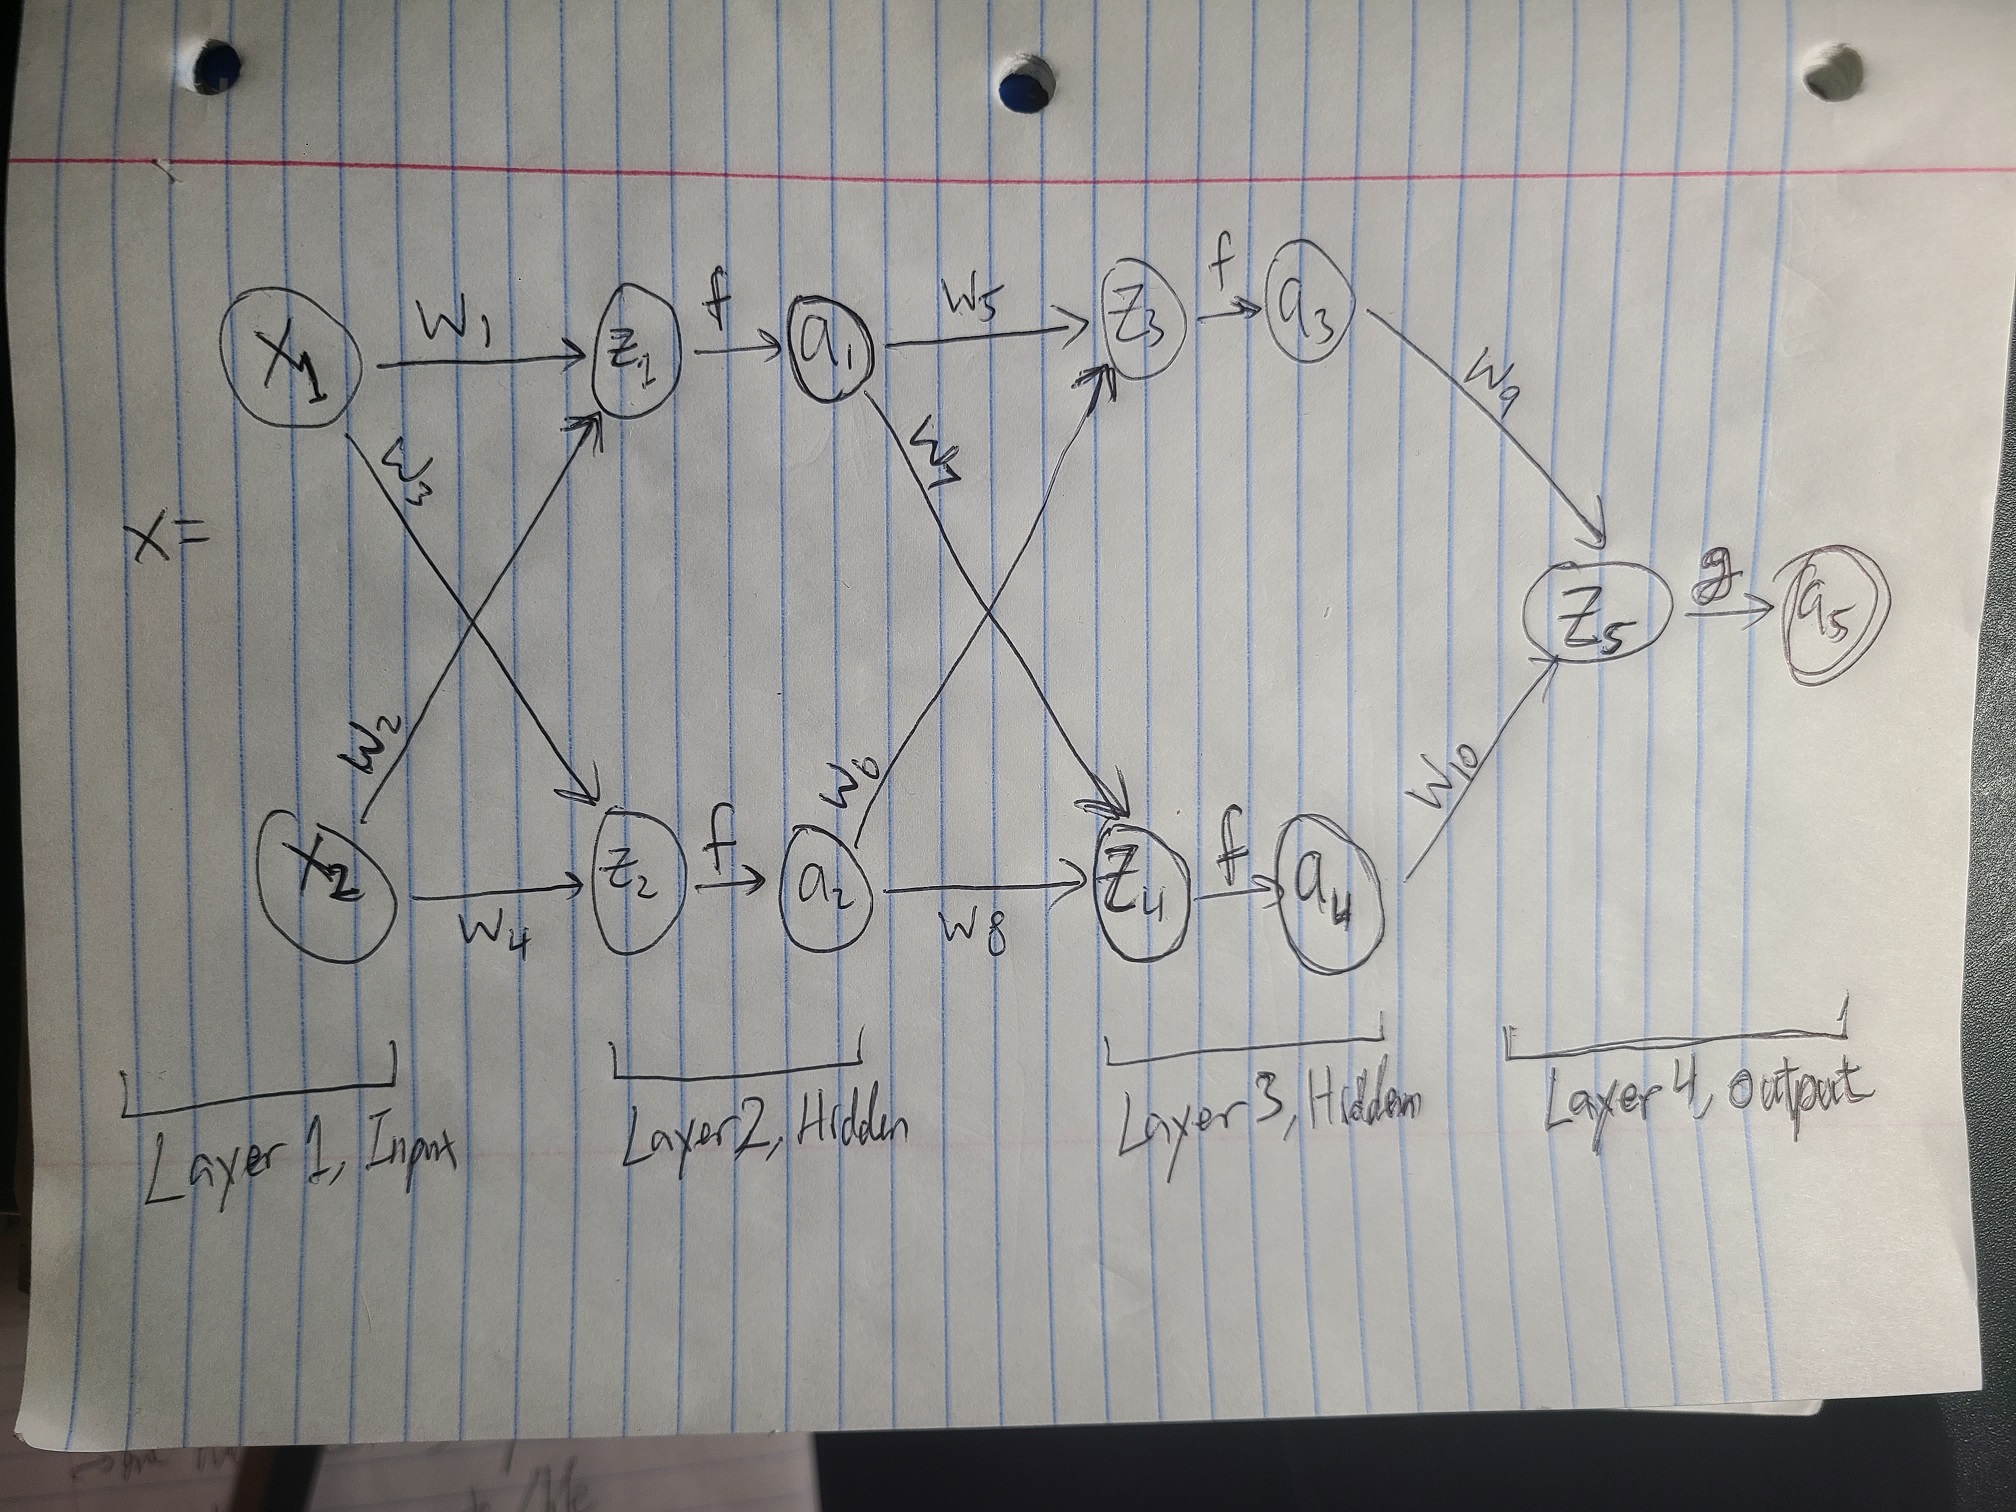
\includegraphics{nn_image.jpg}
\caption{Neural Net Image}
\end{figure}

In this image, we are feeding a single 2-dimensional data point
\(x = (x_1, x_2)\) through a NN to try and get a prediction.

Just like how a signal from your hand travels through many layers of
neurons before finally reaching your brain, \textbf{a neural network
contains multiple layers which process the data and make a prediction}.

Our Neural Network has 4 \textbf{layers}. The input layer, two
``hidden'' layers, and the output layer. Aside from the input and output
layer, all other layers of a neural network are ``hidden'' layers.

Each layer of the NN contains a bunch of cells called \textbf{nodes}.
These are the \(z_i\) the \(a_i\). The \(z_i\) are ``unactivated''
nodes. The \(a_i\) are ``activated'' nodes. The ``unactivated'' nodes
\(z_i\) can be thought of as the dendrite part of the neurons in our
body. They receive signals from nodes in the previous layer.

Some of these \textbf{signals} may be stronger, some may be weaker. The
\textbf{signal strengths} coming from nodes in the previous layer are
controlled by scalar \textbf{weights}, the \(w_i\).

The final aggregated signal that reaches our current layer's node is
just a \textbf{linear combination} of the \textbf{previous nodes} (or
more specifically the values of the nodes) and their respective
\textbf{signal strengths} (i.e.~the \textbf{weights}). So for example,
\(z_1 = w_1x_1 + w_2x_2\).

This aggregated signal is just the value of our (unactivated)
\textbf{node} in our current layer, \(z_i\). The way that a
\textbf{node} in our current layer \(z_i\) decides what
signal/information to pass through is with a function called an
\textbf{activation function}, denoted \(f\) (and \(g\)) in the image.
The function \(f\) takes the ``unactivated'' node as an input, and and
it ouputs an ``activated'' node. So for example, \(f(z_2) = a_2\).

The \textbf{activation function} \(f\) applies a non-linear
transformation to the \(z_i\). Common activation functions include: -
the sigmoid \(a_i = f(z_i) = \frac{1}{1+exp(-z_i)}\), - the hyperbolic
tangent \(f(z_i) = tanh(z_i)\), - the ReLU \(f(z_i) = z_i, z_i > 0\) and
\(0\) otherwise.

\(g\) is just the activation function for the output layer. \(g\) may or
may not equal \(f\). For binary classification problems (i.e.~we want
model to predict a binary outcome), \(g\) is usually the sigmoid
function.

Note that in our NN (and all NN's), it is the ``activated'' node values
\textbf{\(a_i\) that are used as inputs for the next layer of the NN}.
They can be thought of like the axon part of a neuron.

The only exception to this rule is with nodes in the first layer (input
layer). The values of the nodes in this layer are just the values of
each dimension of our data point -- \(x_1\) and \(x_2\). These raw
values are used directly to calculate the aggregate signal for the
(unactivated) nodes in the next layer. In other words, the input data
will not be activated before it is used as a signal for the next layer.
The value of the activated node of the last layer, \(a_5\), gives us the
output, or prediction of the NN.

\textbf{Recap:} Our one data point \(x\) is 2-dimensional. Each
dimension value is used as an input node in the first \textbf{layer} of
our NN. The \(w_i's\) are \textbf{weights}. They are the signal
amplifiers/dampeners that help send the signal from one layer to the
next. The \(z_i's\) and \(a_i's\) make up the \textbf{nodes} for a
\textbf{layer}. The value of each node \(z_i\) is just the aggregate
signal of the previous layer sent to this node. The value
(i.e.~aggregate signal) for \(z_i\) is a \textbf{linear combination} of
the \textbf{nodes \(a_j\) in the previous layer and their respective
weights or signal strengths \(w_j\)}. The \(z_i\) get ``activated'' by
our \textbf{activation function} \(f\). This turns the \(z_i\) into
\(a_i\). \(g\) is also an activation function, specifically for the
output layer. \(g\) may or may not equal \(f\). The \(z_i's\) are like
the dendrites of a neuron. They receive signal from the \(a_k\) nodes in
the previous layer. The \(a_i's\) are like the axons of a neuron. It is
their their values that get sent to the \(z_j\) nodes in the next layer.
The \(z_i\) and \(a_i\) make up a \textbf{layer} of the NN.

\hypertarget{neural-networks-the-forward-pass}{%
\subsubsection{Neural Networks, the Forward
Pass}\label{neural-networks-the-forward-pass}}

Recall our 4-layer NN example.

We have a brand new data point \(x = (x_1, x_2)\). The true outcome of
this data point is \(y\), a binary outcome. We first initialize some
(random) values for the weights \(w_i\). Let's assume our activation
functions \(f\) and \(g\) are both sigmoids,
\(f(x) = \frac{1}{1+exp(-x)}\) Let us calculate what the prediction by
our Neural Net for this data point will be.

\textbf{Question !} Based on the NN structure, write out the values of
\(z_1\) and \(z_2\) as functions of \(x_i's\) and \(w_i's\).

\textbf{Question !!} Write out \(a_1\) and \(a_2\) as functions of the
\(z_i's\). Does \(a_1\) \emph{directly} depend on \(w_2\)? Does \(a_1\)
\emph{indirectly} depend on \(w_2\)? If so, through what? Does \(a_1\)
\emph{indirectly} depend on \(w_4\)? If so, through what?

\textbf{Question !} Write out \(z_3\) and \(z_4\) as functions of
\(a_i's\) and the \(w_i's\). Do \(z_3\) and \(z_4\) \emph{directly}
depend on anything else?

\textbf{Question !} Write out \(z_5\) as a function of \(a_3\) and
\(a_4\). Write out \(a_5\) in terms of \(z_5\).

\textbf{Question !} What do \(w_1\), \(w_2\), \ldots, \(w_{10}\) depend
on? Hint: The is a trick question.

Through this exercise, we performed a ``forward pass'' with our data in
the Neural Network. It is exactly like it sounds. We passed our data
point through every layer of our NN.

In each layer, the neural net took a linear combination of the signals
from the previous layer and then transformed this aggregated signal into
a new signal to pass onto the next layer.

We did this until we finally got \(a_5\), the value of our output layer,
i.e.~the prediction of our NN.

Hooray!

\hypertarget{neural-networks-back-propagation}{%
\subsubsection{Neural Networks,
Back-Propagation}\label{neural-networks-back-propagation}}

\begin{figure}
\centering
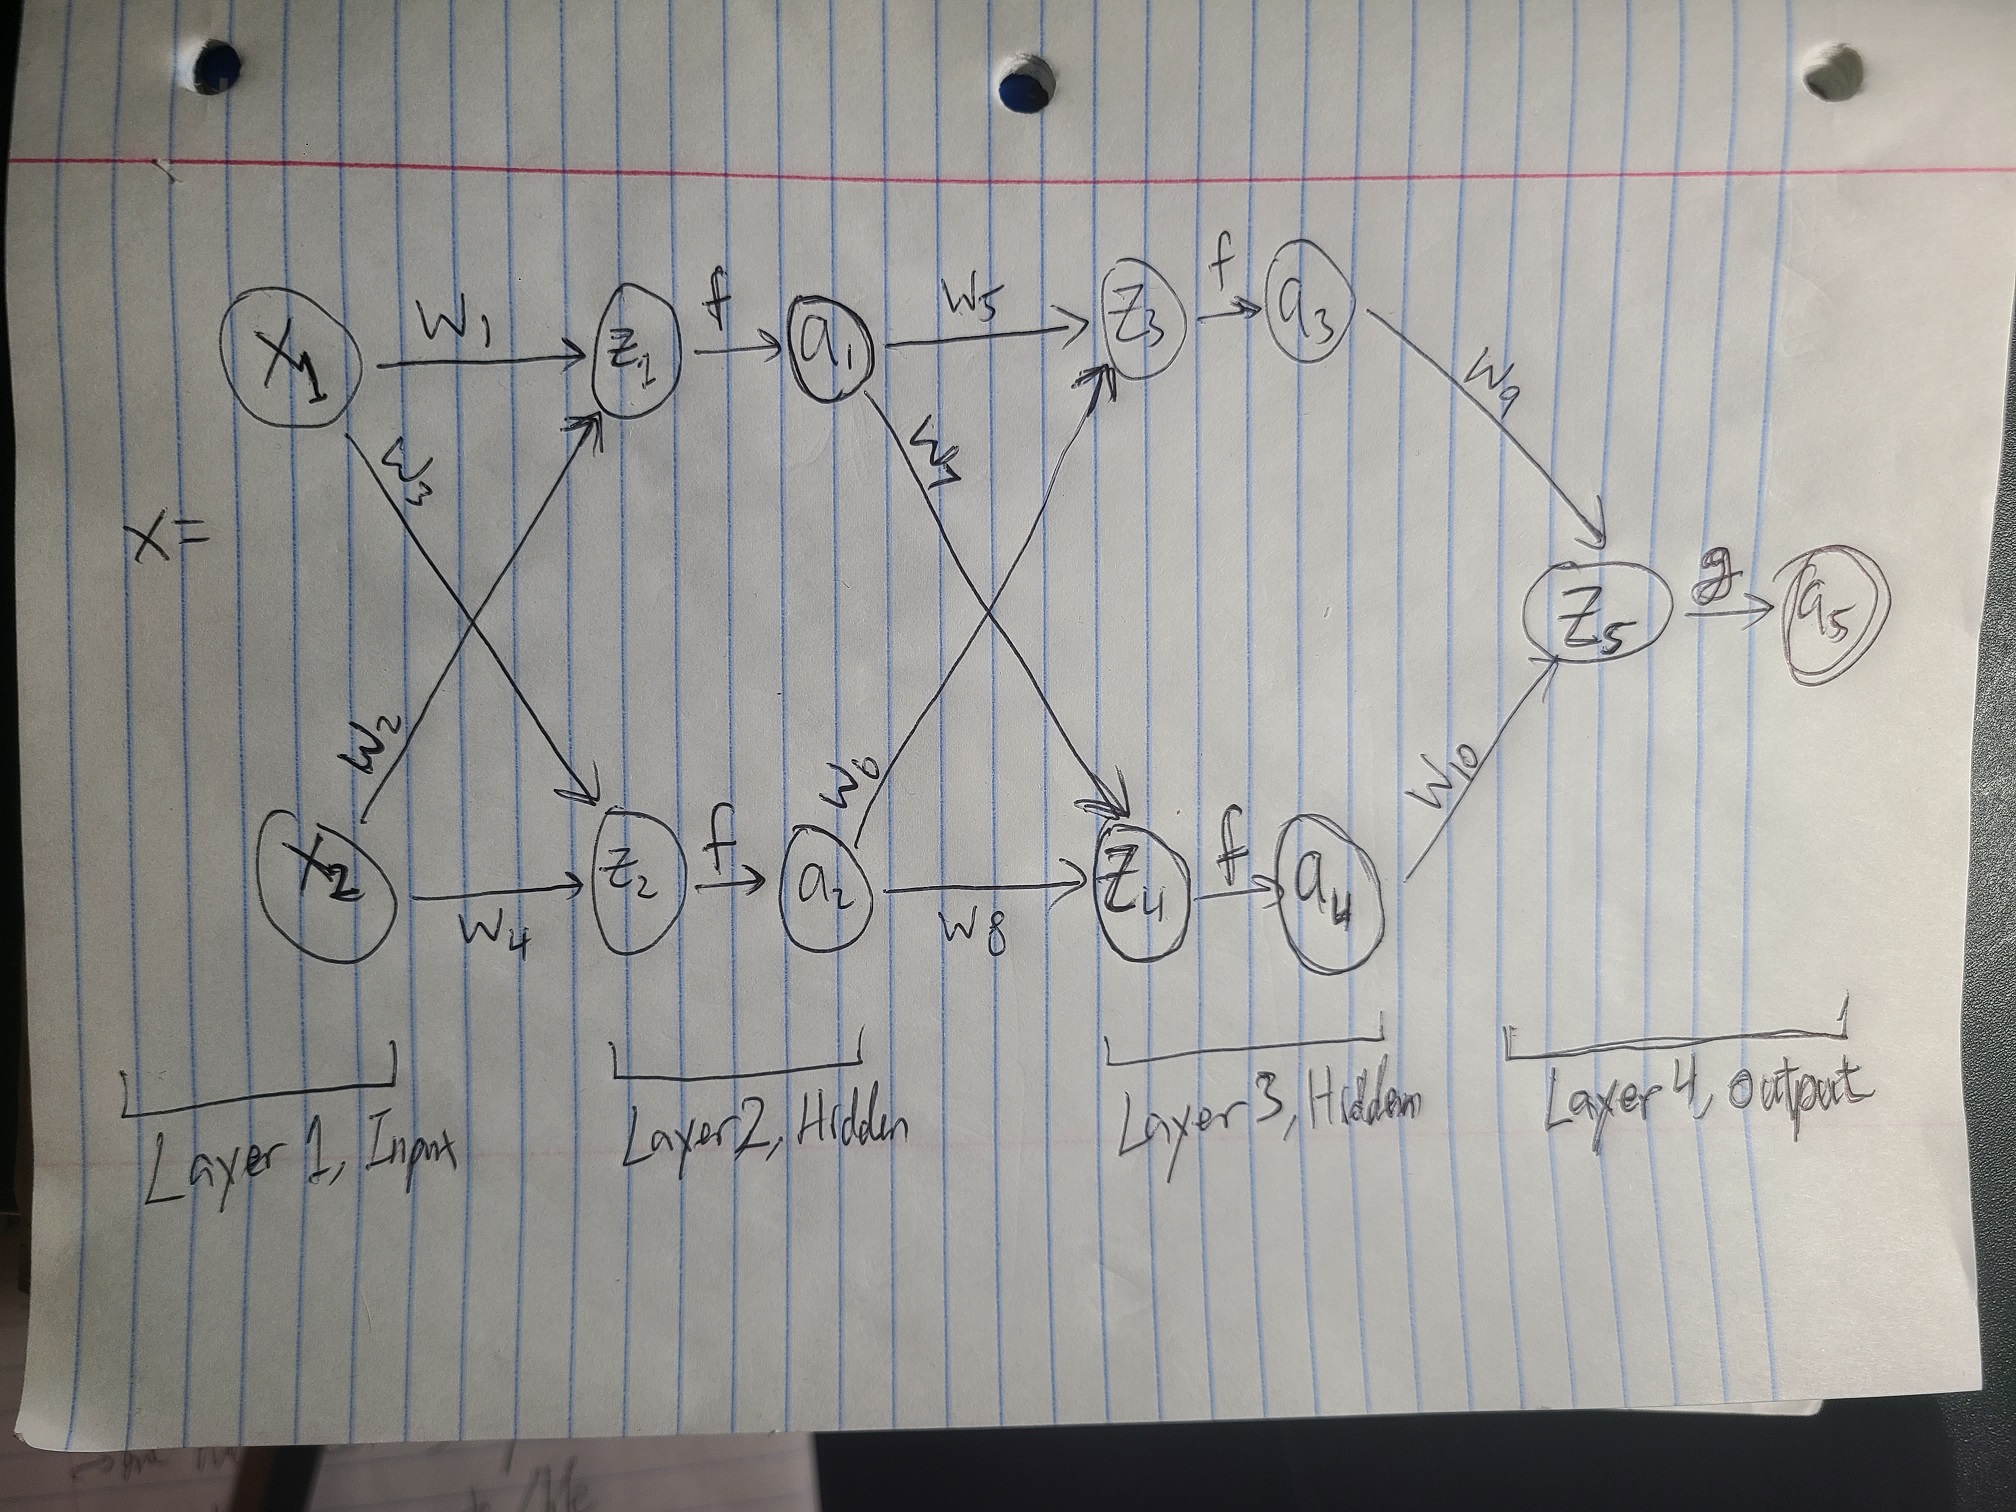
\includegraphics{nn_image.jpg}
\caption{Neural Net Image}
\end{figure}

Perhaps we ``Hooray!''-ed too soon. Recall our 4-layer NN above. In our
setup, we started out by picking random weights \(w_i\) for our NN. But
these weights are probably horrible! Our output \(a_5\), i.e.~our
prediction, probably doesn't even come close to the true outcome of the
data, \(y\).

So, like all ML algorithms, we need to define our model performance
using a cost function. And then we need to tweak our parameters
\(w_i's\) in the right direction get us closer to the minimum of this
cost function.

Let our cost function be the Mean Squared Error. We only have one data
point, so it's really just Squared Error. Lol. In cost function
notation, this is \(C(\theta|y) = (y - a_3)^2\).

What is our \(\theta\), our parameters? For our Neural Net, the
\(w_i's\) are the only parameters that our neural net can tweak when
trying to find the optimal of the cost function for our data. This is
because the \(w_i's\) don't depend on anything else. Unlike the
\(z_i's\) or \(a_i's\), they are not functions of anything. They
just\ldots{} are.

You might wonder, ``What about the number of layers of the NN, or the
number of nodes in each layer, or even the activation functions \(f\)
and \(g\)? Can't we tweak these too?'' Ye we can, but these are the
\emph{hyperparameters} of our Neural Net. Once these hyperparameters are
``set'' in our NN structure, they cannot be changed.

Now that we have established what our \(\theta's\) are, let's substitute
it back into the cost function. So \(C(\theta|y)\) becomes
\(C(w_i's|y) = (a_5 - y)^2\).

Like all ML, we want to improve our model prediction by minimizing our
cost function through Gradient Descent.

Recall the general Gradient Descent formula from earlier,
\(\theta_{new} = \theta_{old} - \alpha \nabla C(\theta_{old})\).

This is a vector representation of Gradient Descent. But a gradient is
the same thing as expressing--in a vector form--the partial derivatives
of our cost function with respect to every single one of our parameters,
our \(w_i's\).

So, to apply GD to minimize the cost function of our NN, we need to
calculate all 10 partials. Assume all activation functions are sigmoids.

Two More Notes: 1) The derivative of a sigmoid function is
\(f'(x) = f(x)(1-f(x))\). 2) Feel free to leave your answers in notation
form as necessary. But for easy-to-calculate derivatives, please try to
provide the derivative value and not the notation.

\textbf{Question !!} Let's start with \(w_9\). Calculate
\(\frac{\partial C(w_i's|y)}{\partial w_9}\) Hint: Use the Chain Rule
(1-dimensional case). Hint: Recall the Forward Pass exercise. How does
\(a_5\) depend on \(w_9\)? Does it depend directly on \(w_5\)? Hint: The
answer is \(2(a_5-y)g(z_5)(1-g(z_5))a_3\). See if you can verify.

\textbf{Question !} Confirm that in our NN structure, the partial with
respect to \(w_{10}\) has a similar setup.

\textbf{Question !!!} Next, let's do \(w_5\). calculate
\(\frac{\partial C(w_i's|y)}{\partial w_5}\). Hint: Use the Chain Rule
(1-dimensional case). Hint: Recall the Forward Pass exercises. How does
\(a_5\) depend on \(w_5\)? Does it depend directly on \(w_5\)? Or does
it depend on things that depend on things that\ldots{} depend on
\(w_5\)? Hint: The answer is
\(2(a_5-y)g(z_5)(1-g(z_5))w_9f(z_3)(1-f(z_3))a_1\). See if you can
verify.

\textbf{Question !} Confirm that in our NN structure, the partials with
respect to \(w_6\), \(w_7\), and \(w_8\) have a similar setup.

\textbf{Question !!!! (CHALLENGE)} Now, let's do \(w_1\). calculate
\(\frac{\partial C(w_i's|y)}{\partial w_1}\). Hint: Use the Chain Rule
(multi-dimensional case). Hint: Recall the Forward Pass exercise. Which
node(s) in the 2nd layer depend(s) on \(w_1\)? Hint: Recall the Forward
Pass exercise. Which node(s) in the 3rd layer depend(s) on \(a_1\)?
Hint: There is a plus sign in the final answer. The first part of the
sum is
\(2(a_5-y)g(z_5)(1-g(z_5))w_9f(z_3)(1-f(z_3))w_5f(z_1)(1-f(z_1))x_1\).
See if you can verify, and also get the second part of the sum.

\textbf{Question !} Confirm that in our NN structure, the partials with
respect to \(w_2\), \(w_3\), and \(w_4\) have similar setups.

Wooohooo! Hooray! You did it, for real this time :-) What you did was
apply the Back-Propagation algorithm layer by layer, by hand, to get the
partials of each weight \(x_i\) of your NN. Nice work again!

As stated above, the vector representation of your partials with respect
to each \(w_i\) is just the gradient of your parameters. In other
words\ldots{} \[
\nabla C(\theta) = \nabla C(w_{1}, w_{2},..., w_{10}) = (\frac{\partial C(w_i's|y)}{\partial w_1}, ..., \frac{\partial C(w_i's|y)}{\partial w_{10}})
\]

Now you can update all 10 weights in your Neural Net using Gradient
Descent, since you solved the gradient :-)

\(\nabla C(w_{1,new}, w_{2,new}, ..., w_{10,new}) = \nabla C(w_{1,old}, w_{2,old}, ..., w_{10,old}) - \alpha \nabla C(w_{1,old}, w_{2,old}, ..., w_{10,old}))\).

Gradient Descent has now tweaked your weights \(w_i's\) in a way that
will improve your prediction for your data point \(x\). Congratulations!
You are one step closer to the optimal Neural Network for your data
point.

\hypertarget{neural-networks-concluding-thoughts}{%
\subsubsection{Neural Networks, Concluding
Thoughts}\label{neural-networks-concluding-thoughts}}

Like all ML models, Neural Networks are trained/optimized by using
Gradient Descent to iteratively find a set of parameters that minimizes
the cost function of the prediction errors of your model.

Gradient Descent requires you to find the gradient of your cost function
with respect to all your parameters. Back-Propagation is precisely that
method to find the gradient Once you solve the gradient, you can then
apply the Gradient Descent algorithm as usual to tweak your parameters
to get to a lower cost function value. And lower cost function means
better performing model.

And that's all there is to it! You have now mastered the fundamentals of
a Neural Network.

Of course, we can make them much more complicated. Let's throw in some
convolutions, or make some networks that don't just move forward in
calculation (i.e.~the ``Forward Pass'' can be a bit more complicated).

However, the essential workhorse in allowing us to optimize a Neural
Network, no matter what flavor, remains the same. Thank you Gradient
Descent and Back-Propagation for keeping me employed :-)

\hypertarget{useful-references}{%
\subsubsection{Useful References}\label{useful-references}}

Chain Rule --
\url{https://www.youtube.com/watch?v=9yCtWfI_Vjg\&ab_channel=Dr.TreforBazett}
Gradient Descent --
\url{https://www.youtube.com/watch?v=IHZwWFHWa-w\&ab_channel=3Blue1Brown}
Back-Propagation Intuition --
\url{https://www.youtube.com/watch?v=Ilg3gGewQ5U\&ab_channel=3Blue1Brown}
Back-Propagation Calculation --
\url{https://www.youtube.com/watch?v=tIeHLnjs5U8\&ab_channel=3Blue1Brown}
Super useful link for understanding Back-Propagation, but generalized to
more layers, more than one data point, and more than one output in the
output layer --
\url{http://ufldl.stanford.edu/tutorial/supervised/MultiLayerNeuralNetworks/}
Another super useful link --
\url{http://www.cs.cornell.edu/courses/cs5740/2016sp/resources/backprop.pdf}

\end{document}
